\documentclass{article}
\usepackage{graphicx}
\usepackage{amsmath}
\usepackage{caption}

\title{Lanczos Resizing and Rotation for Image Transformation}
\author{Kunovics Dávid Zoltán}
\date{\today}

\begin{document}

\maketitle

\section{Introduction}
Image resizing and rotation are fundamental operations in image processing. They are commonly used in computer vision, graphics design, and other fields. The challenge lies in maintaining high-quality visual results while transforming an image, especially when scaling and rotating simultaneously. This document presents a method that employs Lanczos resampling to resize and rotate images in a single sampling process.

\section{Mathematical Model}

\subsection{Lanczos Resampling}
Lanczos resampling is a high-quality interpolation method based on the sinc function. The sinc function is defined as:
\[
\text{sinc}(x) = \frac{\sin(\pi x)}{\pi x}
\]
The Lanczos kernel for resampling with a parameter \(A\) is given by:
\[
w(x) = \text{sinc}(x) \cdot \text{sinc}\left(\frac{x}{A}\right)
\]
where \(x\) is the distance between the pixel center and the sampling point. The parameter \(A\) controls the size of the kernel, and higher values lead to smoother results but require more computation.

\subsection{Rotation Transformation}
To rotate an image by an angle \(\theta\), we use the 2D rotation matrix:
\[
\begin{bmatrix}
x' \\
y'
\end{bmatrix}
= 
\begin{bmatrix}
\cos(\theta) & -\sin(\theta) \\
\sin(\theta) & \cos(\theta)
\end{bmatrix}
\begin{bmatrix}
x \\
y
\end{bmatrix}
\]
where \((x, y)\) are the coordinates of a point in the original image, and \((x', y')\) are the coordinates in the rotated image. The rotation matrix is applied to each pixel in the image to map the rotated coordinates back to the scaled image.

\section{Methodology}

The method combines two main operations:
\begin{enumerate}
    \item \textbf{Scaling:} The image is resized to the destination dimensions using Lanczos resampling, which handles high-quality interpolation.
    \item \textbf{Rotation:} After scaling, the image is rotated using the 2D rotation matrix, adjusting the image size to fit the rotated content.
\end{enumerate}

\subsection{Steps Involved:}
\begin{enumerate}
    \item The input image is first resized to the desired dimensions.
    \item A rotation matrix is applied to rotate the image by the specified angle.
    \item The new bounding box of the rotated image is calculated to adjust the final image size.
    \item Lanczos resampling is used during both scaling and rotation to ensure high-quality interpolation.
\end{enumerate}

\section{Test Cases}

The method was tested with three images to demonstrate its effectiveness. The images were resized and rotated as follows:

\begin{enumerate}
    \item \textbf{Test Case 1:} Resize to 4x with no rotation (0 degrees).
    \item \textbf{Test Case 2:} Resize to 2x and rotate by 45 degrees.
    \item \textbf{Test Case 3:} Resize to 1x and rotate by 90 degrees.
\end{enumerate}

\begin{figure}[h!]
    \centering
    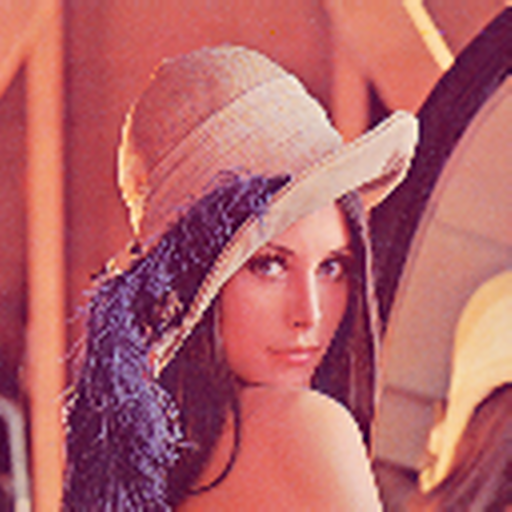
\includegraphics[width=0.4\textwidth]{lena_4.00@0.00.png}
    \caption{Test Case 1: Resized to x4 with no rotation.}
\end{figure}

\begin{figure}[h!]
    \centering
    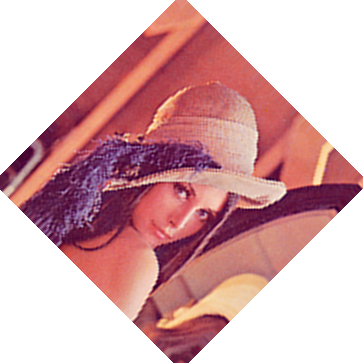
\includegraphics[width=0.4\textwidth]{lena_2.00@45.00.png}
    \caption{Test Case 2: Resized to x2 and rotated by 45 degrees.}
\end{figure}

\begin{figure}[h!]
    \centering
    
\includegraphics[width=0.4\textwidth]{lena_0.50@90.00.png}
    \caption{Test Case 3: Resized to x0.5 and rotated by 90 degrees.}
\end{figure}

\section{Conclusion}

The proposed method efficiently combines resizing and rotation using a single sampling process based on Lanczos resampling. This approach provides high-quality transformations, ensuring sharpness and smoothness in the final image. The test cases demonstrated the versatility of the method for different image sizes and rotation angles.

\end{document}
